%%%%%%%%%%%%%%%%%%%%%%%%%%%%%%%%%%%%%%%%%%%%%%%%%%%%%%%%%%%%%%%%%%%%%%
% 
% LICENSE: Creative Commons Attribution 4.0 International
% © Mohammad-Mohsen Aseman-Manzar, https://asemanmanzar.ir/
% 
% ------------------------------------------------------------------
% Based On LaTeX Template: Curriculum Vitae
%
% Source: http://www.howtotex.com/
% Feel free to distribute this template, but please keep the
% referal to HowToTeX.com.
% Date: July 2011
%
%%%%%%%%%%%%%%%%%%%%%%%%%%%%%%%%%%%%%%%%%%%%%%%%%%%%%%%%%%%%%%%%%%%%%%
\documentclass[paper=a4,fontsize=11pt]{scrartcl} % KOMA-article class

\usepackage[english]{babel}
\usepackage[utf8x]{inputenc}
\usepackage[protrusion=true,expansion=true]{microtype}
\usepackage{amsmath,amsfonts,amsthm}     % Math packages
\usepackage{graphicx}                    % Enable pdflatex
\usepackage[svgnames]{xcolor}            % Colors by their 'svgnames'
\usepackage{geometry}
    \textheight=700px                    % Saving trees ;-)
\usepackage{url}
\usepackage{wrapfig}
\usepackage{tcolorbox}

\frenchspacing              % Better looking spacings after periods
\pagestyle{empty}           % No pagenumbers/headers/footers

%%% Custom sectioning (sectsty package)
%%% ------------------------------------------------------------
\usepackage{sectsty}

\sectionfont{%                        % Change font of \section command
    \usefont{OT1}{phv}{b}{n}%        % bch-b-n: CharterBT-Bold font
    \sectionrule{0pt}{0pt}{-5pt}{3pt}}

%%% Macros
%%% ------------------------------------------------------------
\newlength{\spacebox}
\settowidth{\spacebox}{8888888888}            % Box to align text
\newcommand{\sepspace}{\vspace*{1em}}        % Vertical space macro

\newcommand{\ifNotEmpty}[2]{
        \ifx&#1&%
           % #1 is empty
        \else
        #2
        \fi
        }

\newcommand{\MyName}[1]{ % Name
        \Huge \usefont{OT1}{phv}{b}{n} \hfill #1 %\Huge \fontsize{0}{0}
        \par \normalsize \normalfont}

\newcommand{\MySlogan}[1]{ % Slogan (optional)
        \normalsize \usefont{OT1}{phv}{m}{n}\hfill \textit{#1}
        \par \normalsize \normalfont}

\newcommand{\NewPart}[1]{\section*{\uppercase{#1}}}

\newcommand{\PersonalEntry}[2]{
        \noindent\hangindent=2em\hangafter=0 % Indentation
        \parbox{\spacebox}{        % Box to align text
        \textit{#1}}               % Entry name (birth, address, etc.)
        \hspace{1.5em} #2 \par}    % Entry value

\newcommand{\SkillsEntry}[2]{      % Same as \PersonalEntry
        \noindent\hangafter=0 % Indentation
        \parbox{6em}{        % Box to align text
        \textit{#1}}               % Entry name (birth, address, etc.)
        \hspace{1.5em} #2 \par}    % Entry value

\newcommand{\EducationEntry}[5]{
        \noindent \textbf{#1} \hfill      % Study
        \colorbox{Black}{%
            \parbox{6em}{%
            \hfill\color{White}#2}} \par  % Duration
        \noindent \textit{#3}         % School
        \ifNotEmpty{#4}{
          \par\noindent\hangindent=2em\hangafter=0 \small #4 % Description
        }
        \ifNotEmpty{#5}{
          \par\noindent\hangindent=2em\hangafter=0 \footnotesize #5 % Smaller Description
        }

        \normalsize \par}

\newcommand{\ExperienceEntry}[4]{         % Same as \EducationEntry
        \noindent \textbf{#1} \hfill      % Study
        \colorbox{Black}{%
            \parbox{6em}{%
            \hfill\color{White}#2}} \par      % Duration
        \noindent \textit{#3} \par        % School
        \noindent\hangindent=2em\hangafter=0 \small #4 % Description
        \normalsize \par}

\newcommand{\ExperienceEntryWithTechs}[5]{         % Same as \EducationEntry
        \noindent \textbf{#1} \hfill      % Study
        \colorbox{Black}{%
            \parbox{6em}{%
            \hfill\color{White}#2}} \par      % Duration
        \noindent \textit{#3} \par        % School
        \noindent\hangindent=2em\hangafter=0 \small #4 % Description
        \ifNotEmpty{#5}{
           \\ #5 % Technologies
        }
        \normalsize \par}

\newcommand{\PaperEntry}[6]{         % Same as \EducationEntry
        \noindent \textbf{#1} \hfill      % Study
        \colorbox{Black}{%
            \parbox{#2}{%
            \hfill\color{White}#3}} \par      % Duration
        \noindent \textit{#4} \par        % School
        \noindent\hangindent=2em\hangafter=0 \small #5 % Description
        \ifNotEmpty{#6}{
          \normalsize \par
	 \noindent\hangindent=2em\hangafter=0 \small #6 % Technologies
        }
        \normalsize \par}

% \newcommand{\WorkEntry}[4]{                  % Same as \EducationEntry
%         \noindent \textbf{#1} \hfill      % Jobname
%         \colorbox{Black}{\color{White}#2} \par  % Duration
%         \noindent \textit{#3} \par              % Company
%         \noindent\hangindent=2em\hangafter=0 \small #4 % Description
%         \normalsize \par}

\newcommand{\CourceEntry}[2]{      % Same as \PersonalEntry
        \noindent\hangindent=2em\hangafter=0 % Indentation
        \parbox{4.2\spacebox}{        % Box to align text
        \textit{#1}}               % Entry name (birth, address, etc.)
        \hspace{1em} #2 \tiny / 20 \normalsize \par}    % Entry value


\newtcbox{\techBoxInner}{on line,
        colframe=black,colback=white,
        boxrule=0.5pt,arc=1pt,boxsep=0pt,left=2pt,right=2pt,top=2pt,bottom=2pt}

\newcommand{\techBox}[1]{
        \techBoxInner{#1}}

%%% Begin Document
%%% ------------------------------------------------------------
\begin{document}
% you can upload a photo and include it here...
%\begin{wrapfigure}{l}{0.5\textwidth}
%    \vspace*{-2em}
%        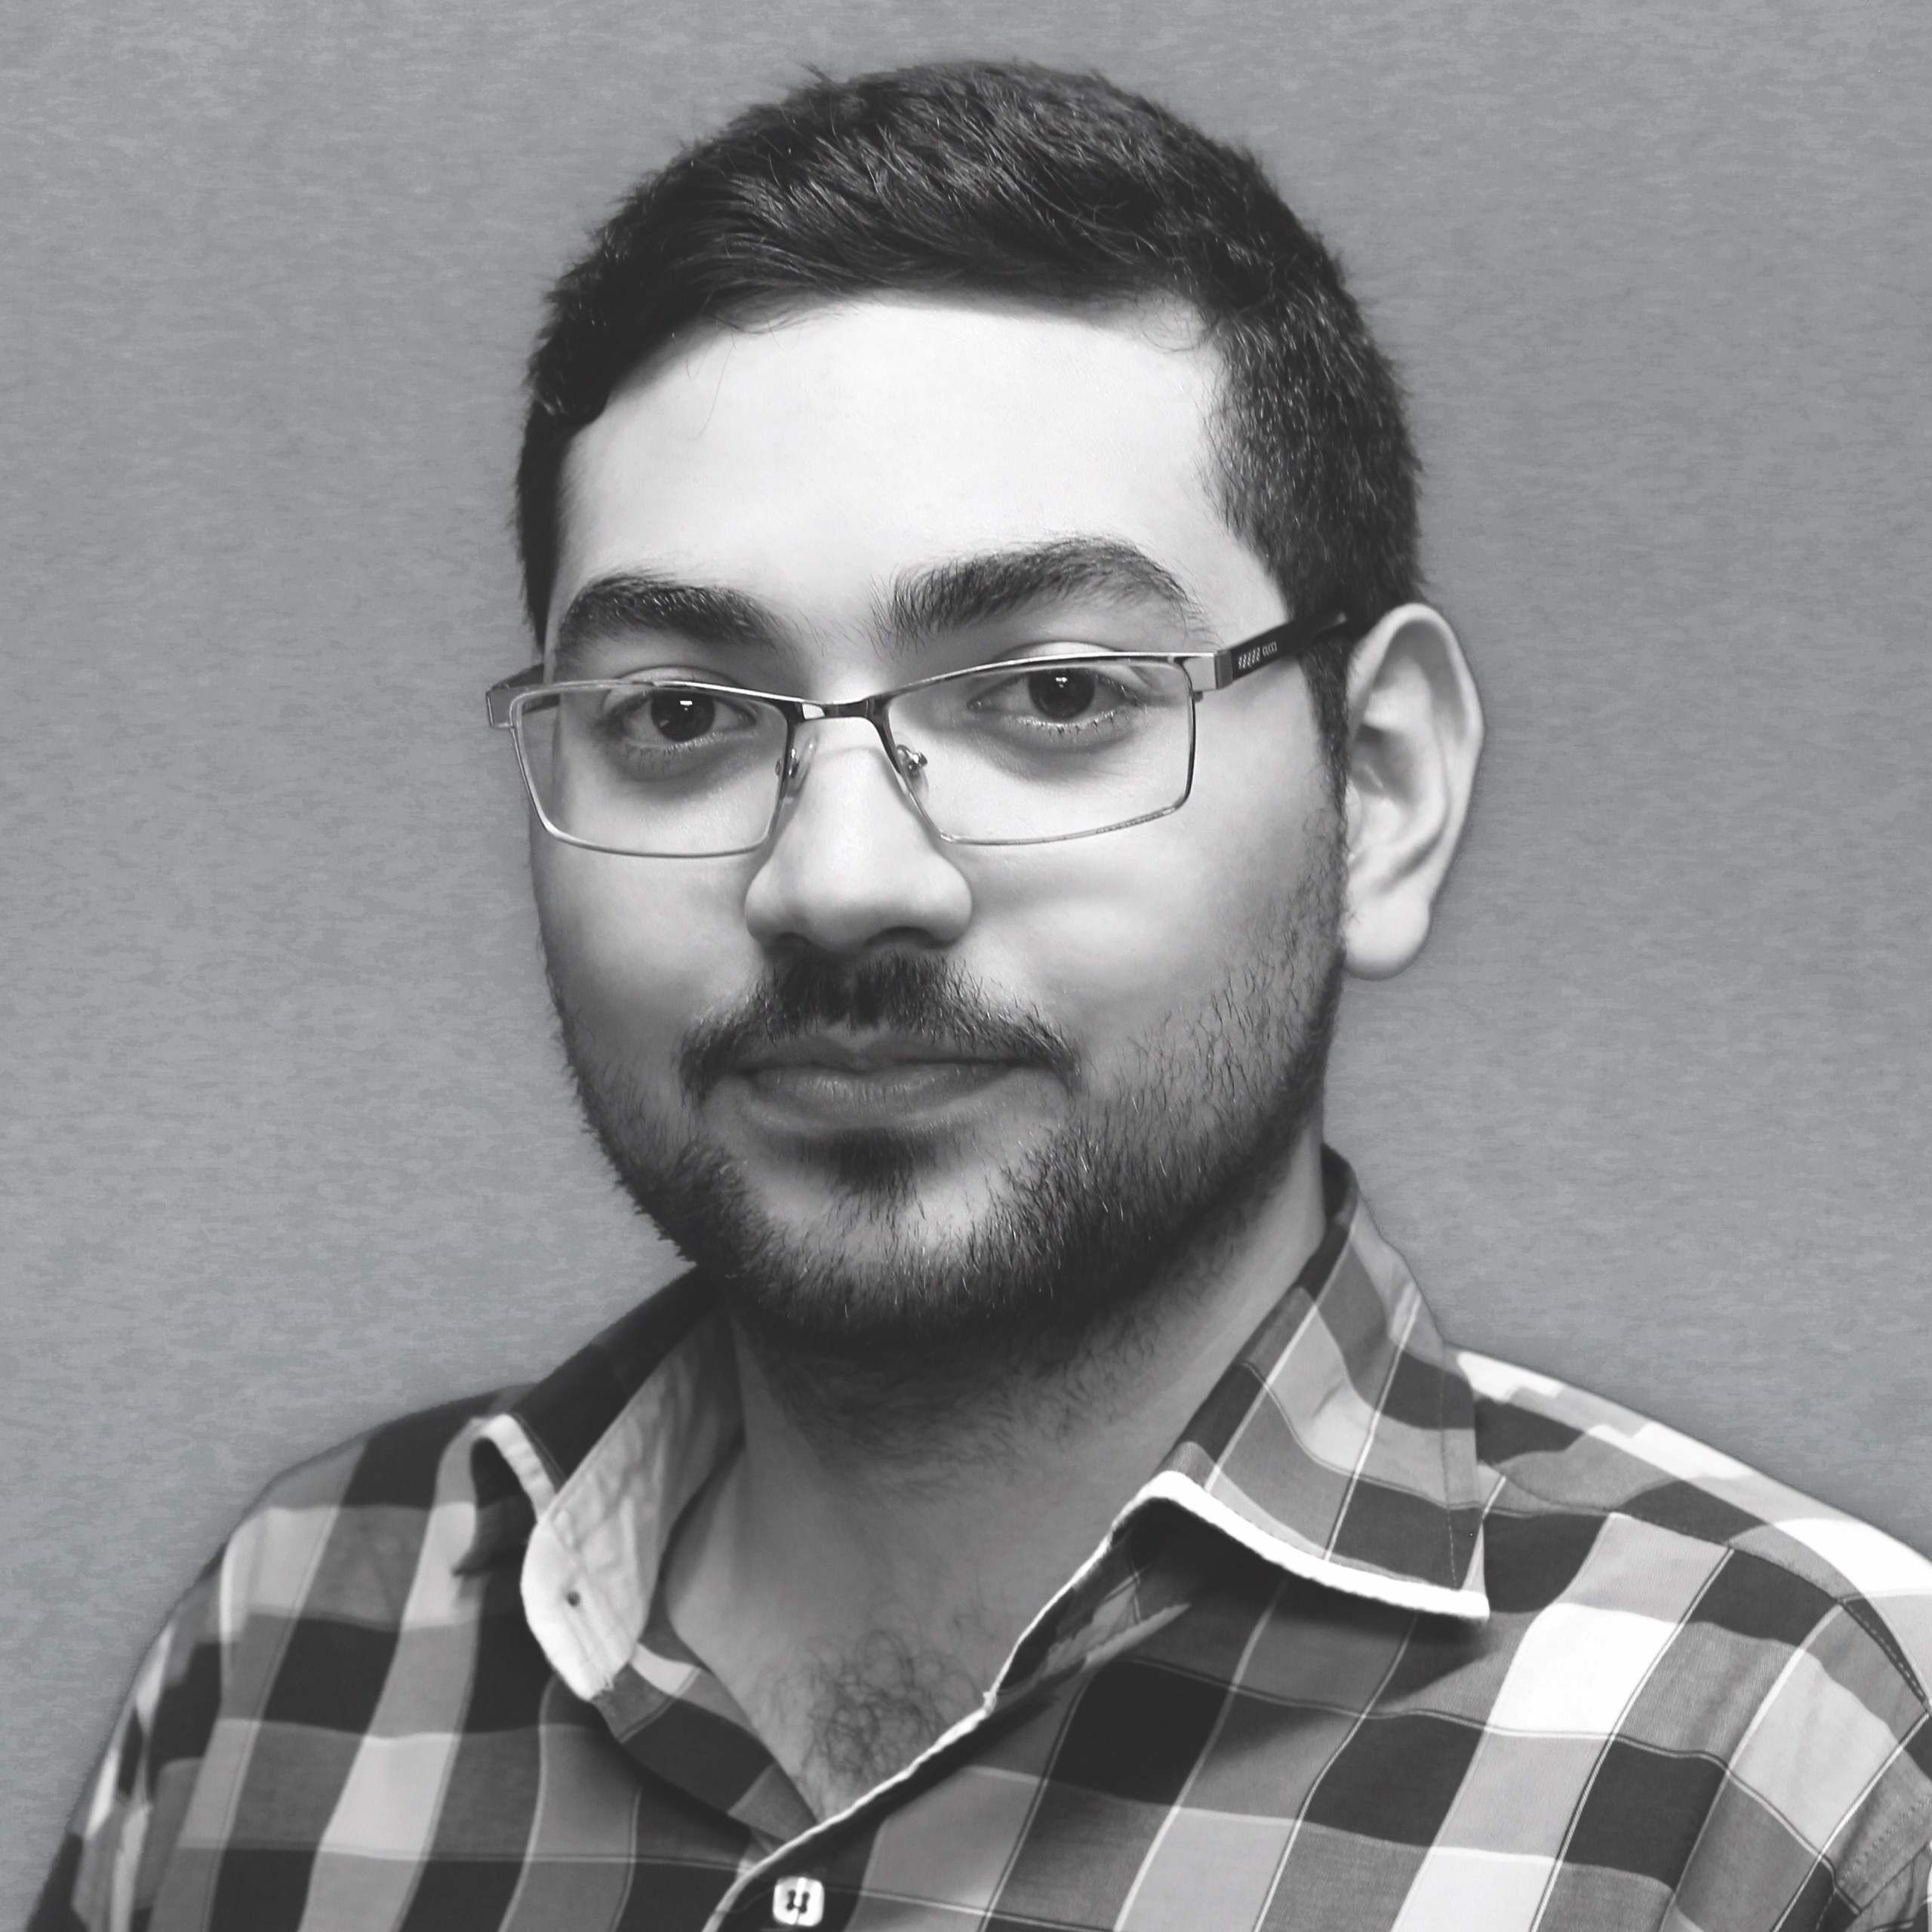
\includegraphics[width=0.15\textwidth]{photo}
%\end{wrapfigure}

%\centerline{In the name of Allah, the Most Gracious, the Most Merciful}
\begin{figure}[ht]
	\centerline{
\includegraphics[width=0.5\textwidth]{besmellah.pdf}}
\end{figure}

\sepspace
\sepspace

\begin{wrapfigure}{l}{0.3\textwidth}
        \vspace*{-3.5em}
        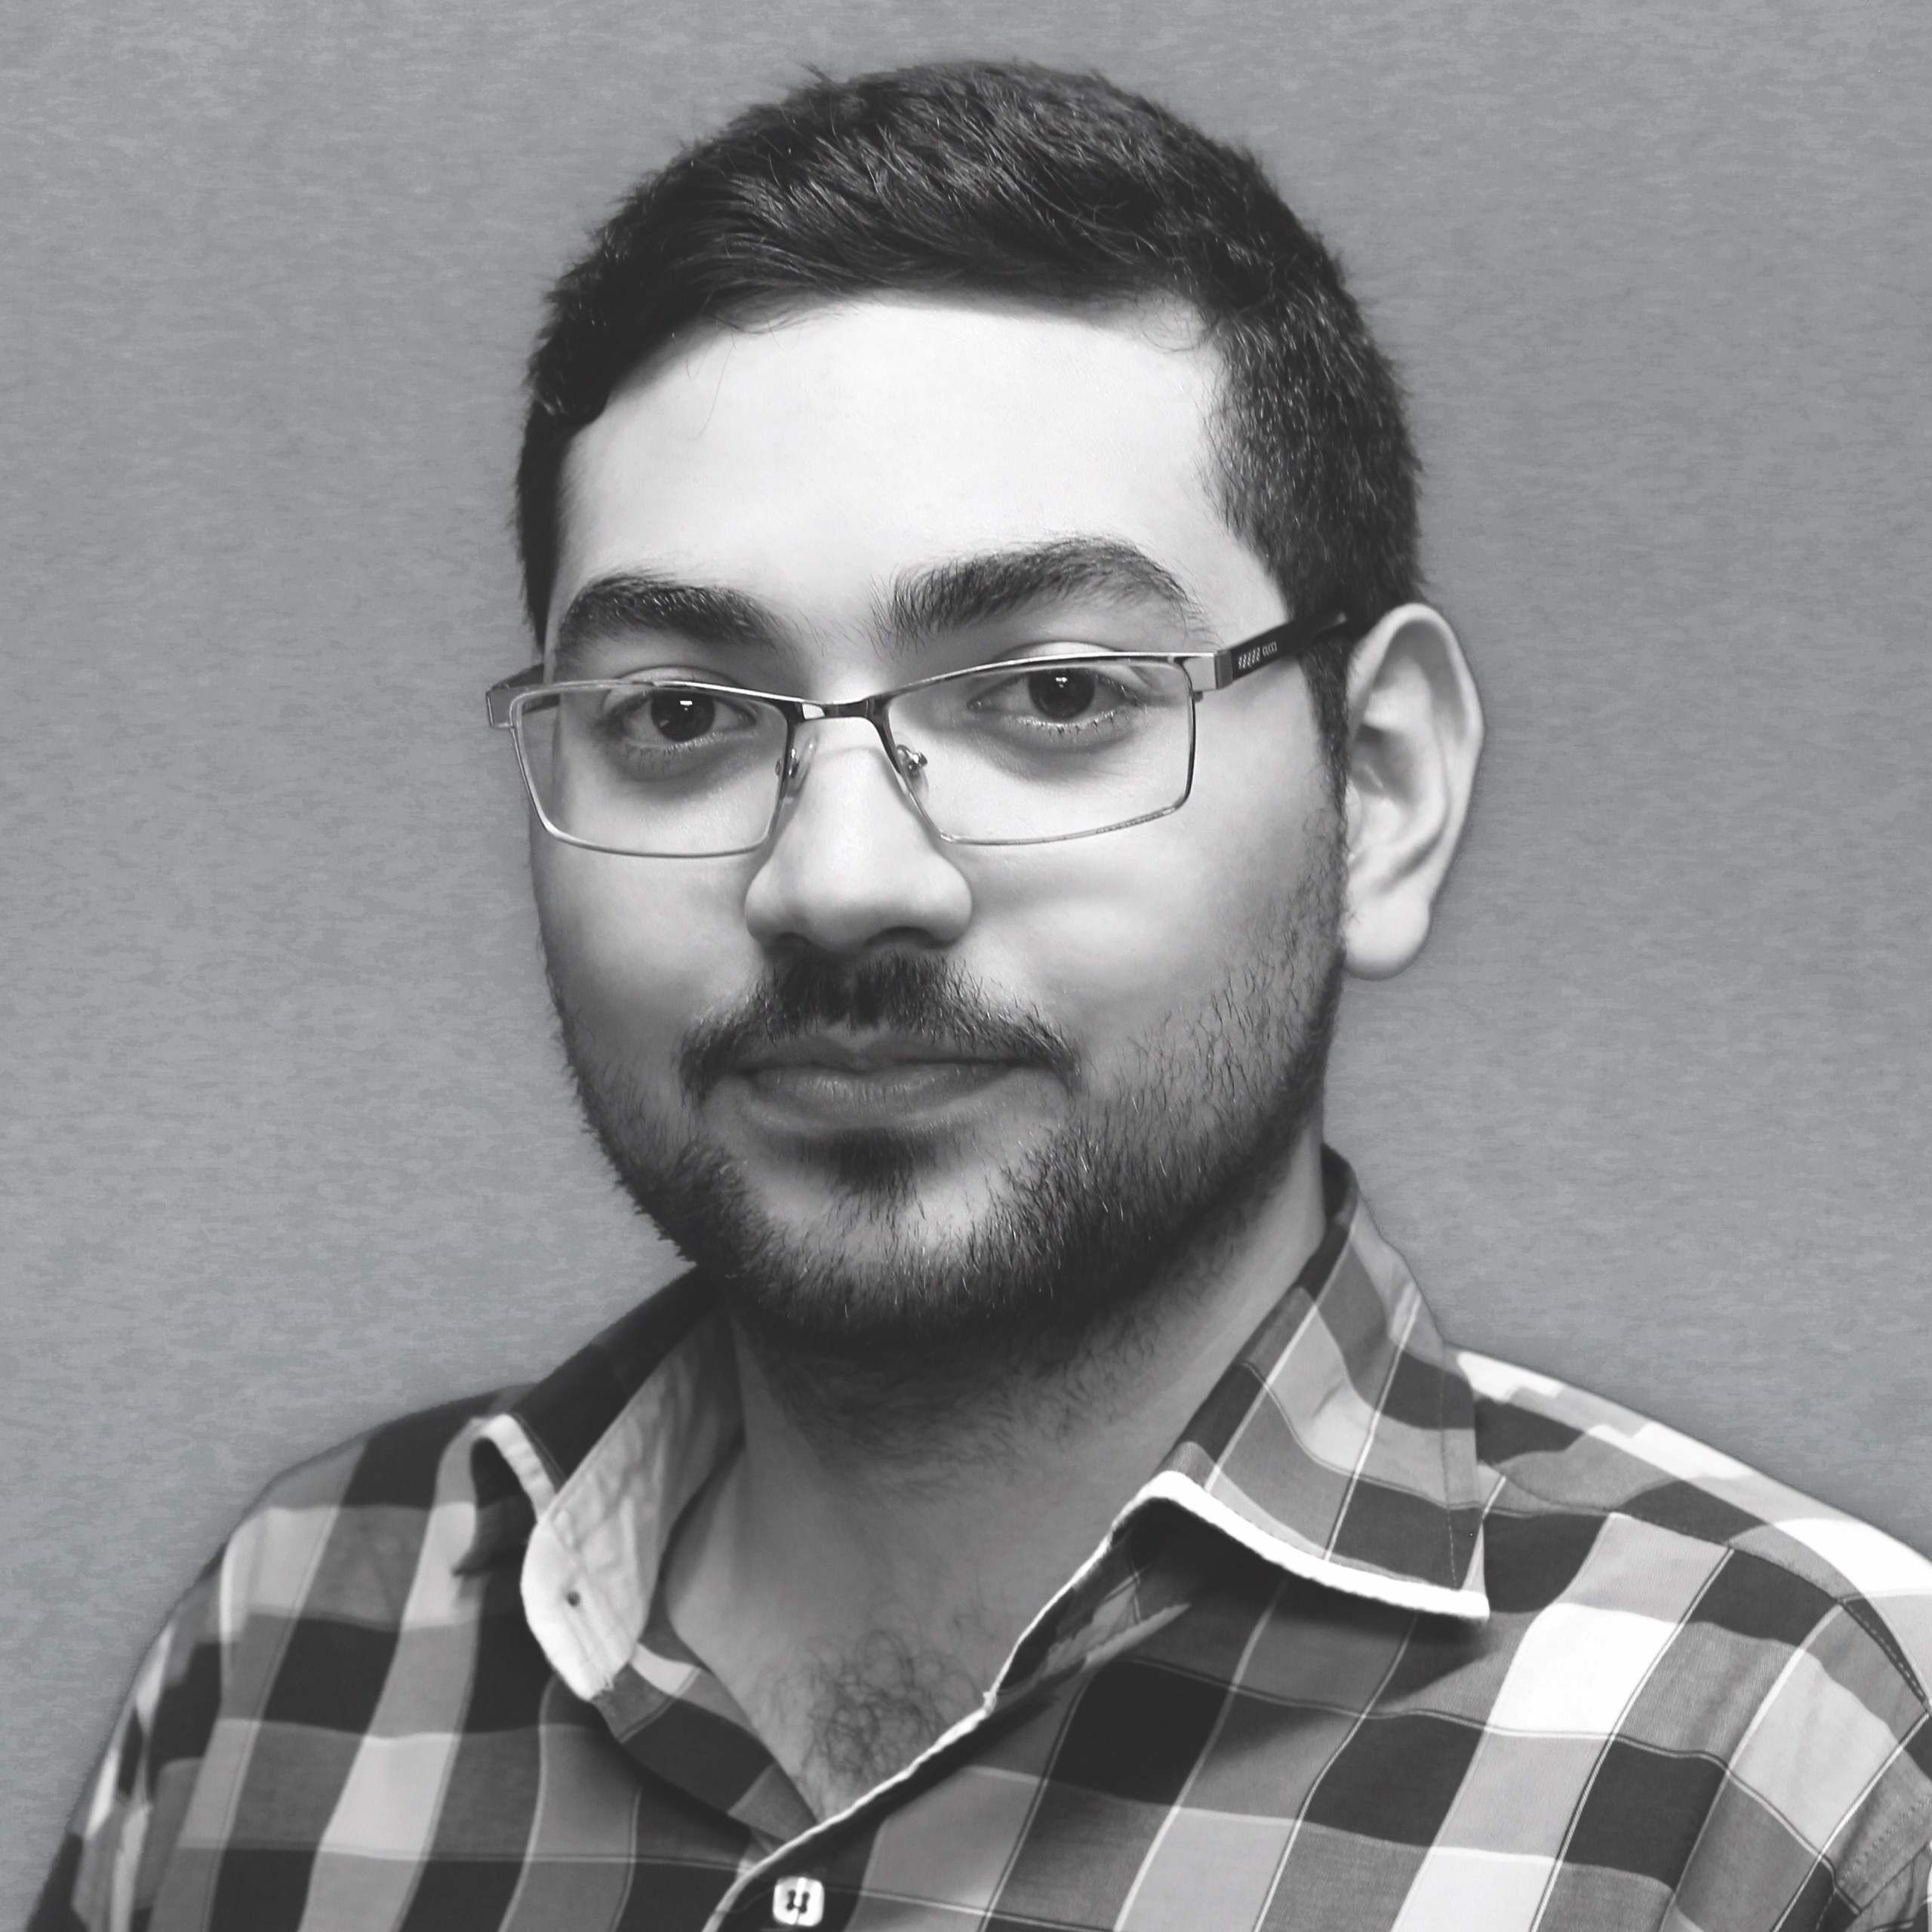
\includegraphics[width=0.2\textwidth]{photo.jpg}
\end{wrapfigure}


\MyName{Aseman Manzar,}
\MyName{Mohammad Mohsen}
\MySlogan{last update: Jan. 20, 2022}

%%% Personal details
%%% ------------------------------------------------------------
\NewPart{Personal details}{}

\PersonalEntry{Birth}{February 10, 1996}
\PersonalEntry{Phone}{+989120728374}
\PersonalEntry{Telegram}{@mohsenasm}
\PersonalEntry{Mail}{\url{m.m.asemanmanzar@gmail.com}}
\PersonalEntry{Website}{\url{https://www.asemanmanzar.ir}}
\PersonalEntry{Resume}{\url{https://www.asemanmanzar.ir/resume.pdf}}
\PersonalEntry{Linkedin}{\url{https://www.linkedin.com/in/asemanmanzar/}}

%%% Education
%%% ------------------------------------------------------------
\NewPart{Education}{}

\EducationEntry
{PhD in Computer Engineering}
{2020-present}
{Sharif University of Technology}
{\underline{Direct Admission}}{\textit{\textbf{Supervisor:} Dr. Mohammad Izadi}}

\sepspace

\EducationEntry
{MSc. in Computer Engineering, Software}
{2018-2020}
{Sharif University of Technology}
{\underline{Direct Admission}, \underline{19.15} GPA}{\textit{\textbf{Project:} Big Data Application Performance Prediction and Cost-based Heterogeneous Resource Recommendation in Cloud
                \newline
                \textbf{Supervisor:} Prof. Ali Movaghar}}

\sepspace

\EducationEntry
{BSc. in Computer Engineering, Software}
{2014-2018}
{Iran University of Science \& Technology}
{\underline{First} Rank, \underline{18.76} GPA}
{\textit{\textbf{Project:} Mixed Performance and Power Consumption Modeling in Virtual Machine Using Coloured Petri Nets
                \newline
                \textbf{Supervisor:} Dr. Mohammad Abdollahi Azgomi}}

\sepspace

\EducationEntry
{Diploma, Mathematics \& Physics}
{2010-2014}
{Allameh Tabatabai School}
{}{}

%%% Work experience
%%% ------------------------------------------------------------
\NewPart{Work experience}{}

\ExperienceEntry
{Senior Software Developer \& System Architect}
{2016-present}
{Hooshravan}
{HooshRavan was born in March 2016 and now its main focus is on "Smart Home Devices." On the market side, The products are known by \textit{Hinava} brand. I joined HooshRavan in 2016 as an \underline{iOS developer}. One and a half years later, I joined the backend team to rewrite the whole \underline{backend} stack to achieve more uptime and stability. Two years later, I wrote the client \underline{web application}.}

%\sepspace
\pagebreak

\ExperienceEntry
{Client/Server Developer}
{2014-2019}
{Elmogame Game Studio}
{Elmogame studio is a game studio founded by Iran University of Science and Technology students in 2013. At the time I was with the team, we published two online android games "Farmuler" and "Footyard" that I was one of the Unity3D developers on these two projects. Besides we were working on another game named "Kalanshahr" that I wrote the backend of this game. This game was later published with the name "NewCity".}

\sepspace

\ExperienceEntry
{iOS Developer}
{2015-2016}
{Hamayeh R\&D}
{Hamayeh was established in 1995, originally aiming at Automation of Control Systems and in less than 5 years of hard work and experience managed to become the major manufacturer of a wide range of different lighting systems equipment. At that time, the R\&D team was working towards making a good Smart Home solution and I was working there to write and maintain its iOS client. }

%%% TA
%%% ------------------------------------------------------------
\NewPart{Teacher Assistant}{}

\ExperienceEntry{Algorithmic Game Theory}{Spring 2022}{Dr. Mohammad Izadi}{}
\ExperienceEntry{Theory of Distributed Systems}{Fall 2021}{Dr. Mohammad Izadi}{}
\ExperienceEntry{Verification of Reactive Systems}{Spring 2020}{Prof. Ali Movaghar}{Textbook: Principles of model checking \textit{written by C. Baier \& JP. Katoen}\newline}
\ExperienceEntry{Principles of Computational Intelligence}{Spring 2018}{Dr. Naser Mozayeni}{}
\ExperienceEntry{Advanced Programming}{Spring 2016}{Dr. Adel Torkaman Rahmani}{}
\ExperienceEntry{Fundamental of Computer Programming}{Fall 2015}{Dr. Adel Torkaman Rahmani}{}

%%% Courses
%%% ------------------------------------------------------------
\NewPart{Selected Courses}{}

\CourceEntry{Advanced Programming}{20}
\CourceEntry{Discrete Mathematics}{20}
% \CourceEntry{Logic Circuits}{19.75}
\CourceEntry{Data Structures}{20}
\CourceEntry{The Theory of Formal Languages and Automata}{20}
\CourceEntry{System Analysis and Design}{20}
\CourceEntry{Software Engineering}{19}
\CourceEntry{Operating Systems}{19.6}
\CourceEntry{Artificial Intelligence and Expert Systems}{20}
\CourceEntry{Computer Networks}{17.7}
\CourceEntry{Software Testing}{20}
\CourceEntry{Formal Methods in Software Engineering}{20}
\CourceEntry{Object-Oriented Analysis and Design}{19.6}
\CourceEntry{Formal Specification and Verification of Programs}{19.0}
\CourceEntry{Computer System Performance Evaluation}{19.3}
\CourceEntry{Theory of Distributed Systems}{19.7}
\CourceEntry{Algorithmic Game Theory}{19.5}
\CourceEntry{Semantic Web}{20}
\CourceEntry{Data Mining}{20}


%%% Publication
%%% ------------------------------------------------------------
\NewPart{Publication}{}

\PaperEntry
{Cost-aware Resource Recommendation for DAG-based Big Data Workflows: Apache Spark Case Study}
{10em}{Accepted; To Appear}
{\underline{Mohammad-Mohsen Aseman-Manzar}, Soroush Karimian-Aliabadi, \newline
        Reza Entezari-Maleki, Bernhard Egger and Ali Movaghar}
{IEEE Transactions on Services Computing}
{}

\sepspace

\PaperEntry
{Fixed-point Iterations Approach to Spark Scalable Performance Modeling and Evaluation}
{10em}{Accepted; To Appear}
{Soroush Karimian-Aliabadi, \underline{Mohammad-Mohsen Aseman-Manzar}, \newline
        Reza Entezari-Maleki, Danilo Ardagna, Bernhard Egger and Ali Movaghar}
{IEEE Transactions on Cloud Computing}
{https://ieeexplore.ieee.org/abstract/document/9573291}

\sepspace

\PaperEntry
{Designing a platform for analysing games' users' data and classification of essential metrics (in persian)}
{7em}{November 2017}
{\underline{Mohammad-Mohsen Aseman-Manzar}, Sarah Aseman-Manzar and Behrooz Minaei}
{1st Digital Games Research Conference (DGRC), https://civilica.com/doc/696919}


%%% Projects
%%% ------------------------------------------------------------
\NewPart{Project}{}

\ExperienceEntryWithTechs
{Hinava Smart Home}
{2016-Present}
{As a Senior iOS/Backend/WebApp Developer \& System Architect}
{Hinava is a smart home system developed in Hooshravan company in Iran.
        It is one of the first and best manufacturers of smart home systems in the country.
        The system in Hinava smart home includes three parts; Hardware devices, Hinava cloud service, and mobile applications. The devices include a central panel which acts as a gateway to our system. The other devices like sensors and actuators are connected to the central panel and through it, they connect to the cloud and user's app on smartphones or tablets.
}
{(iOS:\techBox{Swift}) (WebApp:\techBox{React}) (Backend:\techBox{Docker} \techBox{Docker Swarm} \techBox{CockroachDB} \techBox{Redis} \techBox{Openresty} \techBox{HAProxy} \techBox{Golang} \techBox{Python}  \techBox{Kibana} \techBox{Elasticsearch} \techBox{Grafana} \techBox{Prometheus} \techBox{Kafka} and so on)}

\sepspace

\ExperienceEntryWithTechs
{MSc. Project}
{2018-2020}
{Supervisor: Prof. Ali Movaghar}
{Project Title: Big Data Application Performance Prediction and Cost-based Heterogeneous Resource Recommendation in Cloud}
{\techBox{Spark} \techBox{Hadoop 2.x, 3.x} \techBox{Yarn} \techBox{Linear Programming} \techBox{Performance Prediction} \\
\techBox{TPC-DS Benchmark} \techBox{Gurobi}}

%\sepspace
\pagebreak

%\ExperienceEntryWithTechs
%{BSc. Project}
%{2017-2018}
%{Supervisor: Dr. Mohammad Abdollahi Azgomi}
%{Project Title: Mixed Performance and Power Consumption Modeling in Virtual Machine Using Coloured Petri Nets}
%{\techBox{CPN-Tools} \techBox{ML Language} \techBox{Performance Modeling} \techBox{Power Consumption Modeling}}
%\sepspace

\ExperienceEntryWithTechs
{Gametic - A Game Analytics Tool}
{2016-2017}
{As a Product Manager, Backend Developer}
{Gametic is an analytics tool that is specialized for games. Gametic supports many analytics reports in a user-friendly web-based dashboard in two categories of user reports and financial reports. user reports such as daily active users, users retentions, and sticky factor. financial reports such as ARPU, LTV, and Paid Rate.}
{\techBox{Docker} \techBox{MongoDB Sharded Cluster} \techBox{MongoDB Aggregation Pipeline} \techBox{Redis} \techBox{Nginx} \techBox{Golang} \techBox{Gin Framework} \techBox{Python} \techBox{Vegeta (load testing tool)}}
\sepspace

\ExperienceEntryWithTechs
{Kalanshahr (NewCity) Game}
{2016-2020}
{As a Backend Developer}
{Kalanshahr is an online strategy game that each player manages their city by choosing appropriate defensive strategies to avoid robbery. Each player builds their city and players are usually able to walk around the other players' cities to become aware of their status. Players are also able to watch the inner view of the building in the cities and interact with them.}
{\techBox{Docker} \techBox{PostgreSQL} \techBox{Redis} \techBox{Python} \techBox{Nginx}}
\sepspace

\ExperienceEntryWithTechs
{Footyard Game}
{2015-2017}
{As a Unity3D Developer (Physics, Gameplay, AI, etc.)}
{Footyard is an online football management game with online gameplay. This game is similar to the famous "Soccer Stars" game but with more features. Each player has their team and they are responsible for the team management. It is also possible to find friends and hang out with them.}
{\techBox{Unity3D} \techBox{C\#} \techBox{RabbitMQ}}
\sepspace

\ExperienceEntryWithTechs
{Farmuler Game}
{2015-2016}
{As a Unity3D Developer (Online Gameplay)}
{Farmuler is an online multiplayer farm game for Android devices. The players will compete with each other
to show their skill of time \& resource management, and they will be rewarded as they get to the goals sooner.}
{\techBox{Unity3D} \techBox{C\#} \techBox{Websocket}}
\sepspace


%%% Skills
%%% ------------------------------------------------------------
\NewPart{Skill}{}

\SkillsEntry{Languages}{\textsc{Persian (mother tongue)}}
\SkillsEntry{}{\textsc{English (limited working proficiency, MSRT 70\%)}}
\sepspace

\SkillsEntry{Programming Languages}{\textsc{Python},  \textsc{Go}, \textsc{Swift}, \textsc{C\#}, \textsc{JavaScript}, \textsc{Java}, \textsc{SQL}, \textsc{C/C++}}
\sepspace

\SkillsEntry{Data Stores}{\textsc{Redis}, \textsc{PostgreSQL}, \textsc{MongoDB}, \textsc{CockroachDB}}
\sepspace

% Industry Knowledges
\SkillsEntry{Industry Knowledges}{\{\textsc{Backend}, \textsc{Frontend}, iOS, \textsc{Game}\} \textsc{Dev.}, \textsc{Database Design},}
\SkillsEntry{}{\textsc{Orchestration}, \textsc{Architecture Design}, \textsc{Software Testing}}
\sepspace

\SkillsEntry{Frameworks \& Libraries}{\textsc{Flask}, \textsc{Gin}, \textsc{React}, \textsc{NumPy}, \textsc{PyTorch}}
\sepspace

\SkillsEntry{Other \newline Softwares}{\textsc{Docker}, \textsc{Git}, \textsc{Figma}, \textsc{Unity3D}, \textsc{CPN-Tools},  \LaTeX}
\sepspace


\end{document}
